% Generated by build_conference_paper.py from frozen study outputs and labelled supplements.
\documentclass[conference,letterpaper]{IEEEtran}
\usepackage[T1]{fontenc}
\usepackage[utf8]{inputenc}
\usepackage{cite,amsmath,graphicx,array,booktabs,textcomp}
\usepackage[hidelinks]{hyperref}
\hypersetup{pdftitle={TreeSHAP and LIME for Intrusion Detection: Sensitivity to Masking and Source Holdout},pdfauthor={}}
\begin{document}
\title{TreeSHAP and LIME for Intrusion Detection: Sensitivity to Masking and Source Holdout}
\author{\IEEEauthorblockN{Anonymous submission}}
\maketitle
\begin{abstract}
In one held-out GeNIS scenario, three binary intrusion detectors raise no false alarms yet miss 3,643-3,859 of 4,563 attack records. This failure is obscured by near-perfect scores on the original connection split. We evaluate TreeSHAP and LIME for Random Forest and XGBoost on traceable, class-capped cohorts from official GeNIS and Gotham 2025 releases. On the frozen connection-group split, TreeSHAP yields greater mean predicted-class probability drop in all 24 paired contexts under median/mode replacement. On the same seed-42 records, nearest training donors chosen by retained predictors shrink the GeNIS gaps to 0.0023-0.0109; three of four pointwise mean intervals include zero. Increasing LIME from 350 to 3,500 draws does not close the median/mode gap. Narrower kernels improve fit at the explained input without consistently improving deletion. Across sixteen source-file folds with shared connections purged, we refit 64 models and find predictive failures even for attack types seen in training. Mean median/mode deletion favors TreeSHAP in 62/64 refits, with 2 reversals. Uncapped testing covers 37,941,390 eligible records and retains substantial errors. In an independent 4,415-flow charging-network test, GeNIS-trained protocol/port models flag 34-37\% of benign flows; adding duration and packet count improves source F1 but worsens external F1. These studies distinguish detector transfer from explanation fidelity and do not establish deployment readiness.
\end{abstract}
\begin{IEEEkeywords}Intrusion detection, explainable AI, TreeSHAP, LIME, provenance, group holdout.\end{IEEEkeywords}

\section{Introduction}
An intrusion detector's explanation is meaningful only relative to a specified model, data pipeline and evaluation target. Security machine learning can be distorted by sampling, labels, data leakage and testbed shortcuts \cite{arp}; reconstruction errors in an IDS dataset can materially change class-level results \cite{engelen}. A recent release date does not by itself resolve these problems. We evaluate two openly accessible 2025 author releases, GeNIS \cite{genis_record,genis} and Gotham \cite{gotham_record,gotham}, while retaining source-to-cohort provenance and explicit traffic-group boundaries.

We compare Random Forest (RF) \cite{rf} and XGBoost (XGB) \cite{xgb} for binary and multiclass prediction, and TreeSHAP and LIME on matched records. We ask how the comparison changes with the replacement rule, LIME settings and a source-file split that also purges shared connections. The contribution is empirical evidence about which conclusions persist, supported by traceable source preparation, rather than a new explanation algorithm.

The primary connection split and its statistical families remain frozen. Additional protocols were written before their own execution, after the primary results were known. These extensions diagnose setting dependence within two testbeds and are exploratory.

\section{Related work and evaluation construct}
SHAP assigns additive feature contributions for a specified value function \cite{shap}; TreeSHAP implements efficient tree-ensemble explanations \cite{treeshap}. LIME fits a local surrogate on perturbed neighbors \cite{lime}. Explanation quality has several dimensions rather than a universal scalar: the X-IDS survey \cite{neupane} and security evaluation by Warnecke \emph{et al.} \cite{warnecke} distinguish practical objectives and quantitative criteria. E-XAI compares SHAP and LIME on three IDS datasets using six criteria and Wilcoxon tests \cite{exai}. Gaspar \emph{et al.} investigate system-call sequence explanations, explanation-guided perturbations and perceived interpretability \cite{gaspar}. Therefore, neither using two explainers nor applying quantitative tests is new here.

More recent close comparisons further constrain the contribution. Hermosilla \emph{et al.} compare KernelSHAP and LIME for XGBoost/TabNet using fidelity, stability and feature agreement \cite{forensic}. Nugraha \emph{et al.} study feature selection, retraining, explanation consistency and cost \cite{versatile}. Kalakoti \emph{et al.} evaluate several explainers for deep alert classification, where method rankings depend on the metric \cite{kalakoti}. Their tasks, SHAP variants, backgrounds and perturbation budgets differ from ours; numerical scores cannot be directly ranked across those studies. Almohammadi et al. report weak LIME local fit and missed spoofing attacks in simulated healthcare federation \cite{almohammadi}. Their median-replacement evaluation motivates testing whether the intervention changes the comparison; their scores do not serve as a baseline for these testbeds.

Removal-based evaluation separates the removal mechanism, measured model behavior and summary statistic \cite{covert}. Infidelity and sensitivity likewise depend on perturbation distributions \cite{yeh}, and responsible evaluation requires specifying metric parameters \cite{quantus}. Replacing features can produce inputs outside training support \cite{hase}; dependencies among predictors alter both plausible replacements and attribution interpretations \cite{aas}. Our endpoint is consequently called \emph{deletion fidelity under the stated mask}. It tests a fitted model's response to synthetic predictor replacement, not causal attack relevance. Retraining after removal, as in ROAR \cite{hooker} and E-XAI's descriptive-accuracy analysis, asks a different question.

We extend these designs by comparing fixed rankings under three replacement rules, testing the LIME surrogate budget and locality, and repeating training and explanation under held-out source files. This links the measured explanation advantage to explicit evaluation choices.

\section{Traceable cohorts and frozen holdout}
\subsection{Acquisition and checksum scope}
GeNIS provides simulated enterprise traffic scenarios. We process all eight scenario CSVs at the 5-second flow interval. Both consumed archives match the provider MD5 values; archive and member SHA-256 digests are recorded. Gotham provides packet-level exports from 78 emulated IoT devices. All 78 CSVs and the README are acquired from the official ZIP using HTTP byte ranges. Each member's extracted length and CRC32 match the ZIP directory, and a local SHA-256 is recorded. The complete 23.8-GB Gotham ZIP was not downloaded, so its advertised whole-archive MD5 is \textbf{unverified}. Member checks must not be described as whole-archive verification. Author-generated exports, rather than regenerated raw packet features, are the starting inputs for both datasets.

\subsection{Sampling, labels and preprocessing}
Every selected source member is scanned. Deterministic random priorities with preparation seed 42 retain at most 10,000 records per original eligible label globally, not separately per file. Gotham's 7,670 Unknown-labelled records are excluded before either supervised task; unknown does not mean attack. Binary targets merge only known attacks. Multiclass targets retain the original known categories. Table~\ref{tab:data} describes the resulting cohorts. Class capping changes traffic prevalence and does not model natural alert load.

Audit identifiers, IP/MAC addresses, timestamps, payloads, labels and selected exporter artifacts are excluded from predictors. Retained ports, protocols and traffic statistics may still encode testbed signatures. Constant-column removal, numerical median imputation and categorical encoding/imputation are fitted on training data only. One constant Gotham predictor is removed, leaving 13. No test-set tuning or feature selection is used for the primary models.
\begin{table}[t]\centering
\caption{Prepared cohorts and frozen group holdout}
\label{tab:data}
\footnotesize
\setlength{\tabcolsep}{3pt}\renewcommand{\arraystretch}{1.12}
\begin{tabular}{lrr}\toprule
Property & GeNIS & Gotham \\\midrule
Source records scanned & 3,087,981 & 35,134,281 \\
Selected known-label records & 40,000 & 133,490 \\
Train / test records & 32,346 / 7,654 & 107,120 / 26,370 \\
Train / test groups & 23,487 / 5,872 & 46,615 / 11,654 \\
Predictors after preparation & 69 & 13 \\
Train / test-supported labels & 4 / 4 & 17 / 16 \\
Overlapping train/test groups & 0 & 0 \\
Test patterns seen in training & 379 & 1,914 \\
\bottomrule\end{tabular}
\end{table}
\subsection{Global groups and label support}
GeNIS groups use the provider FlowID globally across scenario files. Gotham groups use a canonical bidirectional IP/transport-port tuple plus protocol globally across device files. Endpoint-equivalent records therefore cannot cross the partition through a different device filename. A GroupShuffleSplit requests 20\% test groups with seed 42. Before fitting, the first of at most 200 candidates covering every eligible label in both partitions is frozen. A label confined to one group is kept entirely in training; there is no row-random fallback. The accepted candidates are 0 for GeNIS and 11 for Gotham.

There are zero shared group keys between training and test. This does not imply all predictor vectors are distinct: 379 GeNIS and 1,914 Gotham test rows exactly match a training predictor vector. The declared primary policy retains these because identical measured predictors may occur in different recorded groups. We assess their influence separately without changing the primary partition. All four GeNIS labels have test support. Gotham has 17 training labels but only 16 supported test labels: CoAP Amplification occupies one group and remains training-only. No test recall or generalization claim is made for it.

\section{Models, explanations and inference}
\subsection{Predictive and diagnostic design}
RF uses 120 trees, maximum depth 18, minimum leaf size 2 and balanced-subsample class weights. XGB uses 160 estimators, maximum depth 7, learning rate 0.08, row/column subsampling 0.85 and class-balancing training sample weights. The same settings are retained across datasets/tasks. Five fitting seeds (42, 52, 62, 72, 82) produce 40 predictive fits. Reported macro-F1 averages only labels with positive test support, with a fixed supported-label set within each task; full class-vocabulary scores remain in the artifacts. A majority classifier and depth-5 tree provide simple baselines on the same holdout. Fitting seeds reuse a single split and do not estimate split uncertainty.

For each of three model seeds (42, 52, 62), both explainers process the same 100 selected records in each dataset/task/model context: 24 paired contexts in total. Selection stratifies class/error diagnostics rather than sampling natural traffic prevalence. The predicted class, including a wrong prediction, is the explanation target. TreeExplainer uses model-based defaults without an explicit background matrix; additivity checking is disabled. LIME uses discretized continuous predictors, 350 perturbations per explanation and a training-only background of at most 5,000 rows stratified by model prediction. These choices are fixed computation budgets, not proof of equal approximation error. A small separate LIME-budget audit is descriptive rather than a convergence guarantee.

Absolute attribution magnitude ranks features for removal. TreeSHAP may explain XGB margin units while LIME explains a probability surrogate; we therefore compare rankings through the same fitted target-class probability, not raw attribution magnitudes. Signed agreement, local surrogate fit, and fixed-model deletion fidelity remain different constructs.

\subsection{Primary endpoint and controls}
Let $f_c(x)$ be the probability of the original predicted class $c$, $r$ an explainer's absolute-magnitude ranking and $M_{k,r}(x;b)$ replace its first $k$ predictors using training numerical medians/categorical modes $b$. The per-record endpoint is
\begin{equation}
\begin{aligned}
D(x,r)&=\frac{1}{|K|}\sum_{k\in K}\left[f_c(x)-f_c(M_{k,r}(x;b))\right],\\
K&=\{1,3,5,10\}.
\end{aligned}
\label{eq:deletion}
\end{equation}
Larger positive drops mean that removing highly ranked predictors more strongly reduces the fitted model's support for that class under this intervention. Negative drops are retained. One seeded random ranking per record and bottom-ranked removal use the same mask/budgets. Random rankings are matched between explainers within context. The random comparison tests ranking utility relative to a weak reference; it is not a no-attack or causal control.

At each budget, records within an explained connection are averaged first; budgets are then averaged into one endpoint per group. Thus every explained group receives equal weight regardless of packet/window count. The paired group difference is $\Delta_g=D_g(\mathrm{TreeSHAP})-D_g(\mathrm{LIME})$. There are 57--95 explained groups per primary context, so 100 records must not be treated as 100 independent connections.

Percentile 95\% intervals use 2,000 paired group bootstrap resamples \cite{efron}. One-sided Wilcoxon signed-rank tests \cite{wilcoxon} assess the declared alternatives TreeSHAP $>$ LIME and top $>$ random. Holm correction \cite{holm} covers all 24 explainer comparisons and, separately, all 48 random-control comparisons. Intervals are per-context, not simultaneous. Signed-rank interpretation relies on the paired group-difference distribution; the post-hoc sign test below checks direction frequency without assuming symmetric magnitudes. Groups may still share campaigns; neither grouping nor correction removes every dependence source. Model seeds are reported separately rather than pooled as independent datasets.

\section{Results}
\subsection{Prediction quality and coverage failures}
Table~\ref{tab:prediction} reports five-seed supported-label macro-F1 and a shallow-tree reference. GeNIS performance is almost perfect, but the depth-5 tree already reaches 0.9906 multiclass F1. A complex model is therefore not automatically necessary on this testbed; an interpretable-model baseline matters \cite{rudin}. Gotham binary scores also approach one, while multiclass scores are substantially lower. Small standard deviations quantify fitting randomness on this partition, not variation over sites or capture periods.
\begin{table}[t]\centering
\caption{Supported-label macro-F1: five-seed mean (SD) and seed-42 shallow-tree baseline}
\label{tab:prediction}
\footnotesize
\setlength{\tabcolsep}{3pt}\renewcommand{\arraystretch}{1.12}
\begin{tabular}{lccc}\toprule
Dataset/task & RF & XGB & Tree \\\midrule
GeNIS bin. & 0.9998 (0.0000) & 0.9998 (0.0001) & 0.9998 \\
GeNIS multi. & 0.9997 (0.0001) & 1.0000 (0.0000) & 0.9906 \\
Gotham bin. & 1.0000 (0.0000) & 0.9999 (0.0000) & 0.9763 \\
Gotham multi. & 0.8755 (0.0005) & 0.8665 (0.0018) & 0.3589 \\
\bottomrule\end{tabular}
\end{table}
The aggregate Gotham result hides important failures. Both RF and XGB have \textbf{zero recall for Mirai C\&C Communication in all five seeds}, despite 358 held-out records. Seed-42 recall for generic C\&C Communication is 0.817 (RF) and 0.439 (XGB), and TCP Scan recall is 0.773 and 0.850. Merlin ICMP Flooding has perfect recall on only three test records; this is weak coverage evidence. CoAP Amplification has no test records. These limitations prevent claims of complete attack-type detection.

The Gotham multiclass training majority is training-only CoAP Amplification, so that baseline scores zero on held-out supported labels. This is a support/prevalence mismatch and should not be used as an unqualified operational improvement claim. The full per-class outputs preserve unsupported labels and seed-specific errors.

\subsection{Primary paired deletion comparison}
TreeSHAP-minus-LIME group means are positive in all 24 primary contexts (0.0570--0.3058), with positive pointwise intervals and Holm-adjusted directional $p<0.05$. Requiring both a positive interval lower bound and corrected $p<0.05$ against random gives 24/24 TreeSHAP and 20/24 LIME contexts. Four Gotham binary LIME intervals cross zero. No primary mean reverses after omitting one explained group. Exact-pattern exclusion removes 379 GeNIS and 1,914 Gotham rows; all paired means remain positive, while Gotham multiclass macro-F1 decreases by about 0.01. These latter checks are post hoc and do not supply independent captures.

\subsection{Replacement and LIME sensitivity}
For both saved rankings on 100 matched records in each of eight seed-42 contexts, we compare median/mode replacement with joint draws from a fixed pool of up to 5,000 training rows. Empirical replacement uses the same 32 uniformly sampled donors for both rankings at every budget per record. Nearest-donor replacement selects 32 rows by retained-feature distance: capped training-scale numeric differences and categorical mismatch, without labels or predictions. We copy removed features jointly from each donor and average target probabilities. Donor hybrids need not be physically valid traffic.

Figure~\ref{fig:mask} shows that GeNIS mean gaps shrink to 0.0023--0.0109 with nearest donors, and 3/4 pointwise mean intervals include zero. All eight nearest-donor means are positive across the two datasets. Across a separate 24-test Holm family, median/mode and joint donors each have 8/8 significant positive signs; nearest donors have 4/8. These exact two-sided tests concern non-tied direction frequency; bootstrap intervals concern mean differences. The two findings are distinct.
\begin{figure}[t]\centering
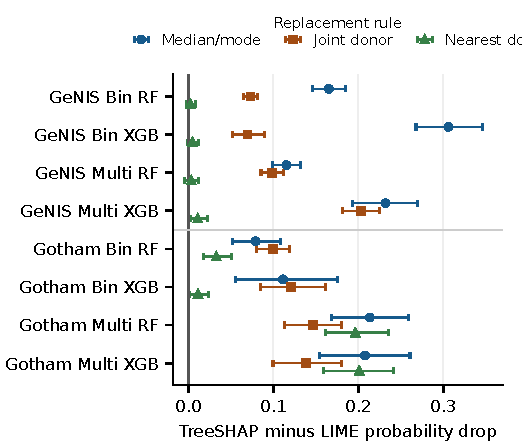
\includegraphics[width=\columnwidth]{figures/mask_sensitivity.pdf}
\caption{Seed-42 paired mean deletion differences by replacement rule and pointwise 95\% connection-bootstrap intervals. Both explainers reuse the same diagnostic records.}
\label{fig:mask}
\end{figure}

Fresh default-neighborhood LIME fits at 350 and 3,500 draws share a fixed training background and per-record seeds. This schedule differs from the primary warm-up. With median/mode deletion, saved TreeSHAP still exceeds LIME-3500 in 8/8 corrected sign tests (separate family of 16 two-sided contrasts). Yet mean absolute surrogate error at the explained input increases in 8/8 contexts, with 3,500-draw context means 0.173--0.779. A larger budget alone does not fix the local fit. At 3,500 draws, a width grid (0.15, 0.35, 0.75 times the square root of the feature count) reuses identical sampled neighborhoods and model outputs, and reproduces the saved 0.75 fits. The narrowest width lowers mean query error in 8/8 contexts but does not eliminate large errors in Gotham multiclass. Under median/mode deletion, TreeSHAP mean gaps remain positive in 16/16 new contrasts, with 13/16 positive signs after separate Holm correction. No width is selected on test performance. Weighted fit scores use different kernel weights and are not a common test distribution.

\subsection{Held-out source files}
We hold out each of eight GeNIS scenario CSVs and eight Gotham bundles of one attack-bearing source plus benign-only sources. Stable filename-hash order and round-robin assignment fix the latter bundles before fitting, covering all 65 represented files. Purging every training row whose group appears in test gives zero shared source files and groups within each fold. We restore candidates removed by the primary constant filter from verified raw row identities, then refit constant filtering and preprocessing on fold training only. RF and XGB reuse the primary hyperparameters and seed 42 for 64 fits; both explainers evaluate 50 matched records per fit at the original median/mode mask and 350 LIME draws.

Table~\ref{tab:transfer} reports macro-F1 over all labels with test support, including labels absent from training; a separate seen-label score restricts records and labels. GeNIS scenario 6 XGB misses 84.5\% of attacks in binary testing and all 3,853 brute-force records in multiclass testing despite training support. Gotham's combined-cycle-1 bundle has 14,242 test rows of CoAP Amplification or UDP Scan, both absent from its multiclass training set. The paired mean deletion difference favors TreeSHAP in 62/64 contexts and LIME in 2/64. Fold results are descriptive: reused groups, overlapping training data and shared testbed mechanisms preclude pooling for inference.
\begin{table}[t]\centering
\caption{Source holdout: all-test-label macro-F1 and paired deletion across eight folds per row}
\label{tab:transfer}
\footnotesize
\setlength{\tabcolsep}{3pt}\renewcommand{\arraystretch}{1.12}
\begin{tabular}{lccc}\toprule
Dataset/task/model & F1 mean [range] & Gap range & Pos. \\\midrule
GeNIS Bin. RF & 0.916 [0.373,1.000] & -0.017 to 0.068 & 7/8 \\
GeNIS Bin. XGB & 0.702 [0.333,0.991] & 0.057 to 0.196 & 8/8 \\
GeNIS Multi. RF & 0.831 [0.471,0.999] & -0.005 to 0.156 & 7/8 \\
GeNIS Multi. XGB & 0.735 [0.465,0.998] & 0.196 to 0.415 & 8/8 \\
Gotham Bin. RF & 0.949 [0.593,1.000] & 0.015 to 0.134 & 8/8 \\
Gotham Bin. XGB & 0.916 [0.591,1.000] & 0.055 to 0.274 & 8/8 \\
Gotham Multi. RF & 0.872 [0.666,0.942] & 0.138 to 0.239 & 8/8 \\
Gotham Multi. XGB & 0.880 [0.654,0.964] & 0.120 to 0.275 & 8/8 \\
\bottomrule\end{tabular}
\end{table}

\subsection{Uncapped scoring and independent capture}
The same 64 saved detectors score all eight GeNIS and 65 assigned Gotham source files without test caps. We exclude Unknown labels and any additional test rows matching fold-training connection keys. Uncapped scoring retains 3,012,335 GeNIS and 34,929,055 Gotham records after label and connection exclusions. Binary macro-F1 spans 0.042-1.000 across GeNIS fold-model contexts and 0.764-1.000 across Gotham contexts. GeNIS scenario 6 XGB misses 10,003 of 11,995 attacks. The expanded test changes class mix and coverage, with no additional training or independent capture.

For external transfer, we fit binary RF and XGB only on the original GeNIS training partition. The official OCPP charging-network capture \cite{ocpp} contributes both Combined partitions as external test only, totaling 4,415 provider-balanced flows. We use protocol and unordered TCP/UDP ports, with a second fixed set adding duration (converted to seconds) and total packet count. No target tuning is used. Table~\ref{tab:external} shows that protocol/port models catch almost all attack-labeled flows but flag over a third of benign flows. Adding duration and counts improves source-test F1 yet worsens external F1. Flow exporters and segmentation differ. This evaluates reduced-feature binary detectors, not external explanation fidelity.
\begin{table}[t]\centering
\caption{Independent OCPP test: misses out of 3,532 attacks; false alarms out of 883 benign flows}
\label{tab:external}
\footnotesize
\setlength{\tabcolsep}{3pt}\renewcommand{\arraystretch}{1.12}
\begin{tabular}{llcccc}\toprule
Set & Model & Source F1 & OCPP F1 & Missed & False alarms \\\midrule
Transport & RF & 0.995 & 0.874 & 5 & 303 \\
Transport & XGB & 0.995 & 0.865 & 2 & 325 \\
+ duration/count & RF & 0.999 & 0.637 & 821 & 381 \\
+ duration/count & XGB & 0.999 & 0.657 & 807 & 338 \\
\bottomrule\end{tabular}
\end{table}
\section{Validity, reproducibility and next evaluation}
\textit{Construct validity:} synthetic replacement can expose model behavior on implausible inputs \cite{slack}. Nearest retained-feature donors are an approximate conditioning sensitivity, not a validated traffic generator. Kernel weighting, correlated predictors, output domains and LIME's discretization limit the comparison to the tested settings. Query fit, in-neighborhood fit and deletion assess different behavior.

\textit{Internal and external validity:} source segregation, group purging, training size and label mix change jointly. The comparison does not identify their individual effects. Class caps and diagnostic selection narrow the populations. Temporal and spatial bias matter in security evaluation \cite{tesseract}; the two original splits reuse the same testbeds. The separate OCPP test does not establish open-world or deployment performance.

\textit{Reproducibility:} pinned environment, acquisition hashes, preparation snapshots, assignments, and per-context artifacts support replay of numerical summaries. No identifying repository link appears in this draft. An anonymous supplement is available subject to venue policy.

\textit{Implications for detector review:} scenario 6 shows why a low false-alarm rate is not a release criterion by itself. Among 1,266 benign and 4,563 attack records, RF, XGB and the shallow tree each produce zero false alarms but miss 3,643, 3,854 and 3,859 attacks, respectively. Before using explanations in alert triage, check attack recall by held-out source with denominators, report original-query surrogate error separately from deletion, and show whether the ranking comparison persists across replacement rules. These are evaluation recommendations; their impact on analyst decisions was not measured.

\section{Conclusion}
Median/mode masking favors TreeSHAP throughout the primary study, but retained-feature donor replacement makes the GeNIS effects much smaller. Larger LIME budgets alone do not improve surrogate fit. Source separation exposes failures for attack types seen in training, despite the original near-ceiling detection scores. A traceable evaluation of explanation rankings must report both the intervention and the scope of the held-out traffic.

\section*{AI assistance disclosure}
OpenAI Codex assisted with literature discovery, source-acquisition tooling, data auditing, experiment orchestration and manuscript drafting/revision. Authors must verify the scientific content, citations, results and venue-policy compliance, and accept responsibility for the final submission. No automated text-origin or similarity score is asserted.

\begin{thebibliography}{99}
\bibitem{arp} D. Arp \emph{et al.}, "Dos and don\textquotesingle ts of machine learning in computer security," in \emph{Proc. USENIX Security Symp.}, 2022, pp. 3971--3988.
\bibitem{engelen} G. Engelen, V. Rimmer, and W. Joosen, "Troubleshooting an intrusion detection dataset: The CICIDS2017 case study," in \emph{Proc. IEEE Security and Privacy Workshops}, 2021, pp. 7--12, doi: 10.1109/SPW53761.2021.00009.
\bibitem{genis_record} M. Silva, D. Pinto, J. Vitorino, J. Gonçalves, E. Maia, and I. Praça, "GeNIS: GECAD Network Intrusion Scenarios," Zenodo, ver. 1.0.0, Feb. 24, 2025, doi: \href{https://doi.org/10.5281/zenodo.14919237}{10.5281/zenodo.14919237}.
\bibitem{genis} M. Silva, D. Pinto, J. Vitorino, J. Gonçalves, E. Maia, and I. Praça, "GeNIS: A modular dataset for network intrusion detection and classification," \emph{Data in Brief}, vol. 60, art. no. 111487, Jun. 2025, doi: \href{https://doi.org/10.1016/j.dib.2025.111487}{10.1016/j.dib.2025.111487}.
\bibitem{gotham_record} O. Belarbi, T. Spyridopoulos, E. Anthi, O. Rana, P. Carnelli, and A. Khan, "A Device-Level IoT Network Traffic Dataset with Distributed Capture and Non-IID Characteristics," Zenodo, ver. v1, Feb. 5, 2025, doi: \href{https://doi.org/10.5281/zenodo.14502760}{10.5281/zenodo.14502760}.
\bibitem{gotham} O. Belarbi, T. Spyridopoulos, E. Anthi, O. Rana, P. Carnelli, and A. Khan, "Gotham Dataset 2025: A Reproducible Large-Scale IoT Network Dataset for Intrusion Detection and Security Research," arXiv:2502.03134, ver. 1, Feb. 5, 2025, doi: \href{https://doi.org/10.48550/arXiv.2502.03134}{10.48550/arXiv.2502.03134}.
\bibitem{rf} L. Breiman, "Random forests," \emph{Machine Learning}, vol. 45, no. 1, pp. 5-32, 2001, doi: \href{https://doi.org/10.1023/A:1010933404324}{10.1023/A:1010933404324}.
\bibitem{xgb} T. Chen and C. Guestrin, "XGBoost: A scalable tree boosting system," in \emph{Proc. ACM SIGKDD}, 2016, pp. 785-794, doi: \href{https://doi.org/10.1145/2939672.2939785}{10.1145/2939672.2939785}.
\bibitem{shap} S. M. Lundberg and S.-I. Lee, "A unified approach to interpreting model predictions," in \emph{Advances in Neural Information Processing Systems}, vol. 30, 2017. [Online]. Available: \href{https://proceedings.neurips.cc/paper/2017/hash/8a20a8621978632d76c43dfd28b67767-Abstract.html}{NeurIPS proceedings}.
\bibitem{treeshap} S. M. Lundberg \emph{et al.}, "From local explanations to global understanding with explainable AI for trees," \emph{Nature Machine Intelligence}, vol. 2, pp. 56-67, 2020, doi: \href{https://doi.org/10.1038/s42256-019-0138-9}{10.1038/s42256-019-0138-9}.
\bibitem{lime} M. T. Ribeiro, S. Singh, and C. Guestrin, "Why should I trust you?": Explaining the predictions of any classifier, in \emph{Proc. ACM SIGKDD}, 2016, pp. 1135-1144, doi: \href{https://doi.org/10.1145/2939672.2939778}{10.1145/2939672.2939778}.
\bibitem{neupane} S. Neupane \emph{et al.}, "Explainable intrusion detection systems (X-IDS): A survey of current methods, challenges, and opportunities," \emph{IEEE Access}, vol. 10, pp. 112392-112415, 2022, doi: \href{https://doi.org/10.1109/ACCESS.2022.3216617}{10.1109/ACCESS.2022.3216617}.
\bibitem{warnecke} A. Warnecke, D. Arp, C. Wressnegger, and K. Rieck, "Evaluating explanation methods for deep learning in security," in \emph{Proc. IEEE Eur. Symp. Security and Privacy (EuroS\&P)}, 2020, pp. 158-174, doi: \href{https://doi.org/10.1109/EuroSP48549.2020.00018}{10.1109/EuroSP48549.2020.00018}.
\bibitem{exai} O. Arreche, T. R. Guntur, J. W. Roberts, and M. Abdallah, "E-XAI: Evaluating black-box explainable AI frameworks for network intrusion detection," \emph{IEEE Access}, vol. 12, pp. 23954-23988, 2024, doi: \href{https://doi.org/10.1109/ACCESS.2024.3365140}{10.1109/ACCESS.2024.3365140}.
\bibitem{gaspar} D. Gaspar, P. Silva, and C. Silva, "Explainable AI for intrusion detection systems: LIME and SHAP applicability on multi-layer perceptron," \emph{IEEE Access}, vol. 12, pp. 30164-30175, 2024, doi: \href{https://doi.org/10.1109/ACCESS.2024.3368377}{10.1109/ACCESS.2024.3368377}.
\bibitem{forensic} P. Hermosilla, S. Berrios, and H. Allende-Cid, "Explainable AI for forensic analysis: A comparative study of SHAP and LIME in intrusion detection models," \emph{Applied Sciences}, vol. 15, no. 13, art. no. 7329, 2025, doi: 10.3390/app15137329.
\bibitem{versatile} B. Nugraha, A. V. Jnanashree, and T. Bauschert, "A versatile XAI-based framework for efficient and explainable intrusion detection systems," \emph{Annals of Telecommunications}, vol. 80, pp. 1095--1120, 2025, doi: 10.1007/s12243-025-01118-9.
\bibitem{kalakoti} R. Kalakoti, R. Vaarandi, H. Bahsi, and S. N\~omm, "Evaluating explainable AI for deep learning-based network intrusion detection system alert classification," arXiv:2506.07882, ver. 1, 2025. [Online]. Available: \url{https://arxiv.org/abs/2506.07882v1}.
\bibitem{almohammadi} K. Almohammadi et al., "An explainable data-local federated learning framework for intrusion detection in connected healthcare systems," Frontiers in Medicine, vol. 13, art. 1989148, 2026, doi: 10.3389/fmed.2026.1989148.
\bibitem{covert} I. C. Covert, S. Lundberg, and S.-I. Lee, "Explaining by removing: A unified framework for model explanation," \emph{Journal of Machine Learning Research}, vol. 22, no. 209, pp. 1-90, 2021. [Online]. Available: \href{https://jmlr.org/papers/v22/20-1316.html}{JMLR 20-1316}.
\bibitem{yeh} C.-K. Yeh, C.-Y. Hsieh, A. S. Suggala, D. I. Inouye, and P. Ravikumar, "On the (in)fidelity and sensitivity of explanations," in \emph{Advances in Neural Information Processing Systems}, vol. 32, 2019. [Online]. Available: \href{https://proceedings.neurips.cc/paper/2019/hash/a7471fdc77b3435276507cc8f2dc2569-Abstract.html}{NeurIPS proceedings}.
\bibitem{quantus} A. Hedstr\"om \emph{et al.}, "Quantus: An explainable AI toolkit for responsible evaluation of neural network explanations and beyond," \emph{Journal of Machine Learning Research}, vol. 24, no. 34, pp. 1--11, 2023.
\bibitem{hase} P. Hase, H. Xie, and M. Bansal, "The out-of-distribution problem in explainability and search methods for feature importance explanations," in \emph{Advances in Neural Information Processing Systems}, vol. 34, 2021.
\bibitem{aas} K. Aas, M. Jullum, and A. L\o land, "Explaining individual predictions when features are dependent: More accurate approximations to Shapley values," \emph{Artificial Intelligence}, vol. 298, art. no. 103502, 2021, doi: 10.1016/j.artint.2021.103502.
\bibitem{hooker} S. Hooker, D. Erhan, P.-J. Kindermans, and B. Kim, "A benchmark for interpretability methods in deep neural networks," in \emph{Advances in Neural Information Processing Systems}, vol. 32, 2019.
\bibitem{efron} B. Efron, "Bootstrap methods: Another look at the jackknife," \emph{Annals of Statistics}, vol. 7, no. 1, pp. 1-26, 1979, doi: \href{https://doi.org/10.1214/aos/1176344552}{10.1214/aos/1176344552}.
\bibitem{wilcoxon} F. Wilcoxon, "Individual comparisons by ranking methods," \emph{Biometrics Bulletin}, vol. 1, no. 6, pp. 80-83, 1945. [Online]. Available: \href{https://www.jstor.org/stable/3001968}{JSTOR 3001968}.
\bibitem{holm} S. Holm, "A simple sequentially rejective multiple test procedure," \emph{Scandinavian Journal of Statistics}, vol. 6, no. 2, pp. 65-70, 1979. [Online]. Available: \href{https://www.jstor.org/stable/4615733}{JSTOR 4615733}.
\bibitem{rudin} C. Rudin, "Stop explaining black box machine learning models for high stakes decisions and use interpretable models instead," \emph{Nature Machine Intelligence}, vol. 1, pp. 206--215, 2019, doi: 10.1038/s42256-019-0048-x.
\bibitem{ocpp} C. Dalamagkas \emph{et al.}, "Federated OCPP 1.6 Intrusion Detection Dataset," Zenodo, 2025, doi: \href{https://doi.org/10.21227/v1f0-9t13}{10.21227/v1f0-9t13}.
\bibitem{slack} D. Slack, S. Hilgard, E. Jia, S. Singh, and H. Lakkaraju, "Fooling LIME and SHAP: Adversarial attacks on post hoc explanation methods," in \emph{Proc. AAAI/ACM Conf. AI, Ethics, and Society}, 2020, pp. 180--186.
\bibitem{tesseract} F. Pendlebury, F. Pierazzi, R. Jordaney, J. Kinder, and L. Cavallaro, "TESSERACT: Eliminating experimental bias in malware classification across space and time," in \emph{Proc. USENIX Security Symp.}, 2019, pp. 729--746.
\end{thebibliography}
\end{document}